\documentclass[aspectratio=169]{beamer}

\usetheme{Boadilla}
\usefonttheme{professionalfonts}
\setbeamertemplate{navigation symbols}{}
\setbeamertemplate{itemize items}[circle]
\setbeamertemplate{enumerate items}[default]
\setbeamertemplate{headline}{}

\usepackage[utf8]{inputenc}
\usepackage[T1]{fontenc}
\usepackage{lmodern}
\usepackage{amsmath}
\usepackage{booktabs}
\usepackage{tabularx}
\usepackage{array}
\usepackage{hyperref}
\usepackage[strings]{underscore}
\usepackage{listings}
\usepackage{tikz}
\usetikzlibrary{arrows.meta,positioning,fit,calc,shapes.geometric}
\usepackage{xcolor}

\definecolor{courseblue}{HTML}{12355B}
\definecolor{coursegold}{HTML}{C98A2E}
\definecolor{courseice}{HTML}{EEF3F8}
\definecolor{coursegreen}{HTML}{2F6B4F}
\definecolor{coursegray}{HTML}{4B5563}
\definecolor{codebg}{HTML}{F7F9FC}
\definecolor{codecomment}{HTML}{5E6C84}
\definecolor{codestring}{HTML}{0B6E4F}

\setbeamercolor{palette primary}{bg=courseblue,fg=white}
\setbeamercolor{palette secondary}{bg=coursegold,fg=white}
\setbeamercolor{palette tertiary}{bg=courseblue,fg=white}
\setbeamercolor{palette quaternary}{bg=coursegold,fg=white}
\setbeamercolor{structure}{fg=courseblue}
\setbeamercolor{frametitle}{bg=courseice,fg=courseblue}
\setbeamercolor{title}{fg=courseblue}
\setbeamercolor{block title}{bg=courseblue,fg=white}
\setbeamercolor{block body}{bg=courseice,fg=black}
\setbeamercolor{normal text}{fg=black,bg=white}
\setbeamercolor{alerted text}{fg=coursegold}

\setbeamerfont{footline}{size=\scriptsize}

\setbeamertemplate{footline}{
  \leavevmode
  \hbox{
    \begin{beamercolorbox}[wd=.33\paperwidth,ht=2.8ex,dp=1.2ex,leftskip=0.8em]{palette primary}%
      University of Trieste
    \end{beamercolorbox}%
    \begin{beamercolorbox}[wd=.49\paperwidth,ht=2.8ex,dp=1.2ex,center]{palette tertiary}%
      \coursename{} \textbar{} \coursecode
    \end{beamercolorbox}%
    \begin{beamercolorbox}[wd=.18\paperwidth,ht=2.8ex,dp=1.2ex,rightskip=0.8em plus1fil]{palette secondary}%
      \insertframenumber{} / \inserttotalframenumber
    \end{beamercolorbox}%
  }
}

\hypersetup{
  colorlinks=true,
  linkcolor=courseblue,
  urlcolor=coursegreen
}

\lstdefinestyle{coursepython}{
  language=Python,
  basicstyle=\ttfamily\footnotesize,
  keywordstyle=\color{courseblue}\bfseries,
  commentstyle=\color{codecomment}\itshape,
  stringstyle=\color{codestring},
  showstringspaces=false,
  columns=fullflexible,
  keepspaces=true,
  frame=single,
  framerule=0.6pt,
  rulecolor=\color{courseblue},
  backgroundcolor=\color{codebg},
  xleftmargin=0.4em,
  xrightmargin=0.4em,
  aboveskip=0.4em,
  belowskip=0.2em
}

\newcommand{\coursename}{Data-driven Systems Engineering}
\newcommand{\coursecode}{440MI / 305SM}
\newcommand{\coursefooter}{}

\newcommand{\learninggoals}[1]{
  \begin{block}{Learning goals}
  #1
  \end{block}
}

\newcommand{\repoactivity}[1]{
  \begin{block}{Repo activity}
  #1
  \end{block}
}

\newcommand{\readinglist}[1]{
  \begin{block}{Papers and materials}
  {\footnotesize #1}
  \end{block}
}

\newcommand{\coursecontextframe}[5]{
  \begin{frame}{Course Map and Running Cases}
  \centering
  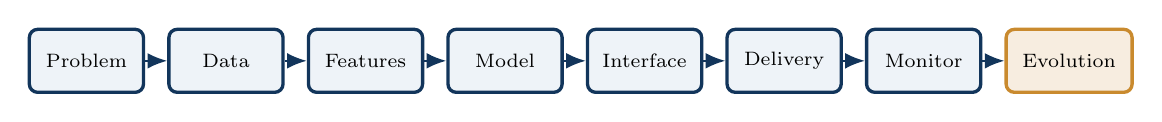
\begin{tikzpicture}[node distance=0.28cm]
  \node[flowbox, minimum width=1.45cm, minimum height=0.8cm] (problem) {\scriptsize Problem};
  \node[flowbox, minimum width=1.45cm, minimum height=0.8cm, right=of problem] (data) {\scriptsize Data};
  \node[flowbox, minimum width=1.45cm, minimum height=0.8cm, right=of data] (features) {\scriptsize Features};
  \node[flowbox, minimum width=1.45cm, minimum height=0.8cm, right=of features] (model) {\scriptsize Model};
  \node[flowbox, minimum width=1.45cm, minimum height=0.8cm, right=of model] (interface) {\scriptsize Interface};
  \node[flowbox, minimum width=1.45cm, minimum height=0.8cm, right=of interface] (delivery) {\scriptsize Delivery};
  \node[flowbox, minimum width=1.45cm, minimum height=0.8cm, right=of delivery] (monitor) {\scriptsize Monitor};
  \node[accentbox, minimum width=1.6cm, minimum height=0.8cm, right=of monitor] (evolution) {\scriptsize Evolution};
  \foreach \a/\b in {problem/data,data/features,features/model,model/interface,interface/delivery,delivery/monitor,monitor/evolution} {
    \draw[arrow] (\a) -- (\b);
  }
  \end{tikzpicture}

  \vspace{0.5em}
  \begin{block}{Today in the course}
  \textbf{Focus:} #1

  \textbf{Bridge:} #2
  \end{block}

  \begin{columns}[T]
  \column{0.48\textwidth}
  \begin{block}{Fraud case}
  {\footnotesize #3}
  \end{block}
  \column{0.48\textwidth}
  \begin{block}{Pasteurization case}
  {\footnotesize #4}
  \end{block}
  \end{columns}

  \vspace{0.3em}
  {\footnotesize \textbf{Course thread:} #5}
  \coursefooter
  \end{frame}
}

\newcommand{\classclosingframe}[4]{
  \begin{frame}{From This Class to the Next}
  \begin{block}{What stays with us}
  #1
  \end{block}

  \begin{columns}[T]
  \column{0.48\textwidth}
  \begin{block}{Project use}
  {\footnotesize #2}
  \end{block}
  \column{0.48\textwidth}
  \begin{block}{Next connection}
  {\footnotesize #3}
  \end{block}
  \end{columns}

  \vspace{0.3em}
  {\footnotesize \textbf{Course thread:} #4}
  \coursefooter
  \end{frame}
}

\tikzset{
  flowbox/.style={
    rounded corners=3pt,
    draw=courseblue,
    fill=courseice,
    very thick,
    minimum width=2.2cm,
    minimum height=0.9cm,
    align=center,
    font=\small
  },
  accentbox/.style={
    rounded corners=3pt,
    draw=coursegold,
    fill=coursegold!15,
    very thick,
    minimum width=2.2cm,
    minimum height=0.9cm,
    align=center,
    font=\small
  },
  arrow/.style={
    -{Latex[length=2.5mm,width=2mm]},
    thick,
    draw=courseblue
  }
}


\title{Class 20: Model Deployment and Prediction Serving}
\author{\coursename}
\date{}

\begin{document}

\frame{\titlepage \coursefooter}

\begin{frame}{Agenda}
\begin{itemize}
\item From a trained artifact to a callable, running service.
\item Flask as a service layer, Streamlit as a presentation layer.
\item The serving architecture already present in this repository.
\item Serving patterns and production concerns beyond a single demo.
\item Closing the Data-Driven block and opening the road into MLOps.
\end{itemize}
\coursefooter
\end{frame}

\begin{frame}{Learning goals}
\learninggoals{
\begin{itemize}
\item Explain the roles of APIs and dashboards in exposing a trained model.
\item Compare Flask and Streamlit and know when each is the right tool.
\item List the minimum quality requirements for a credible prediction service.
\item Recognize which production serving concerns this course's demos do not yet address.
\end{itemize}
}
\coursefooter
\end{frame}

\coursecontextframe
{Turning a model artifact into a served, callable, and observable system.}
{This is the last class of the Data-Driven block: everything from data type, through encoding, features, tuning, and evaluation, converges here into one deployable service boundary.}
{The fraud case becomes a Flask scoring endpoint, `Class6\_model\_api.py`, callable by other services or analysts.}
{The pasteurization case pairs a Flask streaming API with a Streamlit dashboard hub, `streamlit/Main.py`, so sensor state and predictions stay visible together.}
{From Class 21 onward, the course treats these served systems as full software engineering objects: requirements, architecture, delivery, and monitoring.}

\begin{frame}{A model creates value only through an interface}
\begin{itemize}
\item A trained model that nobody can call or interpret has limited practical value, however strong its offline metrics.
\item Interfaces make predictions available to users, services, and operational workflows.
\item The interface also shapes trust: input checks, response format, and clarity all matter.
\end{itemize}
\coursefooter
\end{frame}

\begin{frame}{Flask and Streamlit play different roles}
\begin{tabularx}{\textwidth}{>{\bfseries}l X}
Flask & Best for programmable endpoints over HTTP, such as `POST /predict` or a streaming route. \\
Streamlit & Best for a fast interactive UI: demos, dashboards, or exploratory interfaces. \\
Together & A common pattern is Flask for the backend service and Streamlit for the human-facing interface. \\
\end{tabularx}
\coursefooter
\end{frame}

\begin{frame}{Repository serving architecture}
\centering
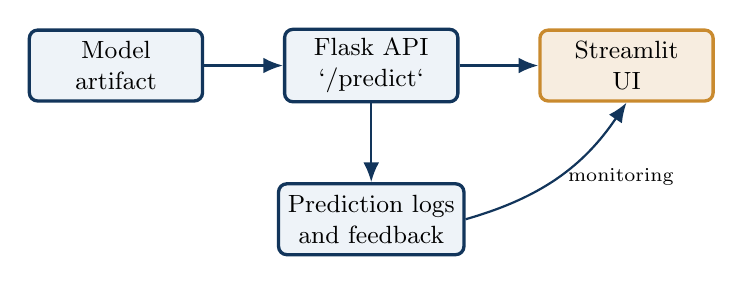
\begin{tikzpicture}[node distance=1cm and 1cm]
\node[flowbox] (model) {Model\\artifact};
\node[flowbox, right=of model] (api) {Flask API\\`/predict`};
\node[accentbox, right=of api] (ui) {Streamlit\\UI};
\node[flowbox, below=of api] (logs) {Prediction logs\\and feedback};
\draw[arrow] (model) -- (api);
\draw[arrow] (api) -- (ui);
\draw[arrow] (api) -- (logs);
\draw[arrow, bend right=20] (logs.east) to node[right, font=\scriptsize] {monitoring} (ui.south);
\end{tikzpicture}
\coursefooter
\end{frame}

\begin{frame}[fragile]{Repository example: the fraud scoring endpoint}
\begin{lstlisting}[style=coursepython]
model = pickle.load(open("notebooks/best_random_forest_model.pkl", "rb"))

@app.route("/")
def index():
    return jsonify({"message": "Model API running"}), 200

@app.route("/predict", methods=["POST"])
def predict():
    data = request.get_json(force=True)
    features = np.array(data["features"]).reshape(1, -1)
    pred = model.predict(features)[0]
    return jsonify({"prediction": int(pred)})
\end{lstlisting}
\begin{itemize}
\item This is the complete serving logic of `Class6\_model\_api.py`: load once at startup, expose one prediction route.
\item It is deliberately small so students can see exactly what a minimal service boundary contains, and what it is still missing.
\end{itemize}
\coursefooter
\end{frame}

\begin{frame}{What a better API should include}
\begin{itemize}
\item A clear input schema, instead of trusting `data["features"]` to always be well-formed.
\item Error handling for malformed or incomplete requests.
\item Stable JSON output with prediction and confidence where appropriate.
\item Logging hooks for later monitoring and debugging.
\item Health or status endpoints for operational checks.
\end{itemize}
\coursefooter
\end{frame}

\begin{frame}[fragile]{Repository example: the dashboard hub}
\begin{lstlisting}[style=coursepython]
st.set_page_config(
    page_title="440MI - Machine Learning Dashboard",
    page_icon=":robot:",
    layout="wide",
    initial_sidebar_state="expanded"
)

st.title("Machine Learning Streamlit Hub")
st.markdown("""
Welcome to the 440MI + 305SM Course.
This interface automatically discovers all available modules
inside the pages/ directory and allows you to navigate between them.
""")
\end{lstlisting}
\begin{itemize}
\item `streamlit/Main.py` is the single entry point that Streamlit's multipage mechanism uses to discover every dashboard in `pages/`.
\item One hub, many served views: fraud scoring, pasteurization streaming, and online learning all live behind it.
\end{itemize}
\coursefooter
\end{frame}

\begin{frame}{Serving patterns in production}
\begin{tabularx}{\textwidth}{>{\bfseries}l X}
Batch scoring & Predictions computed periodically over a stored dataset, not on demand. \\
Online request-response & A client calls an endpoint and waits synchronously for one prediction, as in `Class6\_model\_api.py`. \\
Streaming serving & Predictions computed continuously over an incoming event stream, as in the pasteurization case. \\
\end{tabularx}
\coursefooter
\end{frame}

\begin{frame}{Production serving concerns this repo's demos do not cover}
\begin{itemize}
\item Latency budgets and load testing under concurrent requests.
\item Model versioning and safe rollback if a new artifact regresses.
\item Schema and input validation enforced before the model is ever called.
\item Observability: structured logs, request tracing, and alerting on failure rates.
\end{itemize}
\begin{block}{Why this matters now}
These are exactly the gaps that motivate the software engineering and MLOps material starting next class.
\end{block}
\coursefooter
\end{frame}

\begin{frame}{From a demo service to a production deployment}
\centering
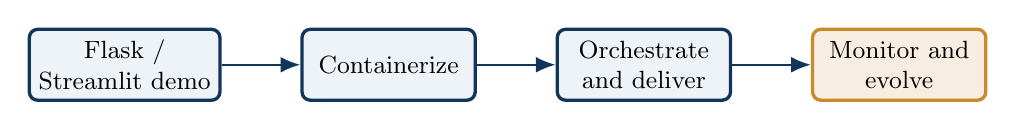
\begin{tikzpicture}[node distance=1cm and 1cm]
\node[flowbox] (demo) {Flask /\\Streamlit demo};
\node[flowbox, right=of demo] (container) {Containerize};
\node[flowbox, right=of container] (orchestrate) {Orchestrate\\and deliver};
\node[accentbox, right=of orchestrate] (monitor) {Monitor and\\evolve};
\draw[arrow] (demo) -- (container);
\draw[arrow] (container) -- (orchestrate);
\draw[arrow] (orchestrate) -- (monitor);
\end{tikzpicture}
\vspace{0.4em}
\begin{itemize}
\item Every arrow here is a topic the MLOps block develops in depth, starting from Class 21.
\end{itemize}
\coursefooter
\end{frame}

\begin{frame}{Repository connections}
\repoactivity{
\begin{itemize}
\item `Class6\_model\_api.py` is the minimal Flask serving example for the fraud case.
\item `streamlit/Main.py` is the dashboard hub that presents fraud, pasteurization, and streaming pages together.
\item `pasteurization/serving.py` shows the same serving concerns applied to a continuous stream instead of a single request.
\end{itemize}
}
\coursefooter
\end{frame}

\begin{frame}{Readiness checklist before calling a model ``served''}
\begin{itemize}
\item Can the service reject a malformed request without crashing?
\item Is the exact preprocessing used at inference identical to what was used in training?
\item Is there any record of which model version answered a given request?
\item Would a teammate other than the author know how to redeploy this service?
\end{itemize}
\coursefooter
\end{frame}

\begin{frame}{Discussion prompt}
\begin{block}{Question}
`Class6\_model\_api.py` returns a bare 0/1 prediction with no schema, confidence, or logging. Is it production-ready?
\end{block}
\begin{itemize}
\item This is deliberately the same tension raised across evaluation (Class 17) and now serving: a working demo is not the same as a dependable system.
\end{itemize}
\coursefooter
\end{frame}

\begin{frame}{Papers and materials}
\readinglist{
\href{https://flask.palletsprojects.com/en/stable/}{Flask documentation};\
\href{https://docs.streamlit.io/}{Streamlit documentation};\
\href{https://12factor.net/}{The Twelve-Factor App};\
\href{https://research.google/pubs/pub46555/}{Sculley et al., Hidden Technical Debt in Machine Learning Systems};\
\href{https://www.oreilly.com/library/view/practical-mlops/9781098103002/}{Practical MLOps}.
}
\coursefooter
\end{frame}

\classclosingframe
{\begin{itemize}
\item A served model is a small software system: an interface, a preprocessing contract, and an operational surface, not just a `.pkl` file.
\item Flask and Streamlit solve complementary problems: programmable endpoints versus human-facing presentation.
\item The gaps in this course's demo services (validation, versioning, observability) are not oversights; they are exactly what the MLOps block exists to close.
\end{itemize}}
{Project teams should now be able to point at their own model artifact and describe, concretely, how it would be called, by whom, and what could go wrong.}
{Class 21: Intervention Cybertec opens the MLOps block, moving from this course's own demo services into full software engineering practice for data products.}
{The Data-Driven block ends where the MLOps block begins: at the boundary where a model becomes a system other people depend on.}

\end{document}
